\documentclass{article}
\usepackage{formats}
\usepackage{graphicx}
%\usepackage[ansinew]{inputenc}

\title{Projet de fin de module - Mixture of Experts (MoE)}
\author{Autheur: Ludovic Andrieu}

\begin{document}

\maketitle

\begin{abstract}
{\em The paragraph corresponding to the summary must be written with 10-point letter, in italics. The word {\bf Abstract} must be centered, and separated three lines from the last author's address. Between the title and the first author leave a space of two lines.}

\end{abstract}

\section{FORMAT GENERAL INSTRUCTIONS (12-point, bold)}
The works must be in paper format of 21 cm x 29.7 cm.
The text must be written in Times New Roman at 10 points, and at two
columns, with a total width of 16 cm; Each column must have
a width of 7.6 cm, with a space between columns of 0.8 cm. The text
it will have a simple line spacing and it must be justified. Leave
a line between paragraphs.

The upper margin should be 2.5 cm and the lower margin should be 3 cm. The margins
left and right should be 2.5 cm.

\section{SECTIONS, NOTES, CITES, FIGURES, EQUATIONS, TABLES AND REFERENCES (12-point, bold)}

\subsection{SECTIONS AND SUBSECTIONS}

\subsubsection{Subsection}

If there were more subsections, they would have the same format as this subsection.
Both the titles of the sections and those of the subsections are with
indentation and aligned to the left.

\subsection{FOOTNOTES}

Do not include header or footer of page.

\subsection{CITATION}

Citation within the text should include the reference number between
square brackets, for example \cite{bibli1}.

\subsection{FIGURES}

All the figures must be centered and clear. The number of the
figure and the legend will always appear at the bottom of the
figure. Each figure must be numbered correlatively and must be
referenced in the text. Leave a line between the text of the paragraph
and the figure.

\begin{figure}[htbp]
\centerline{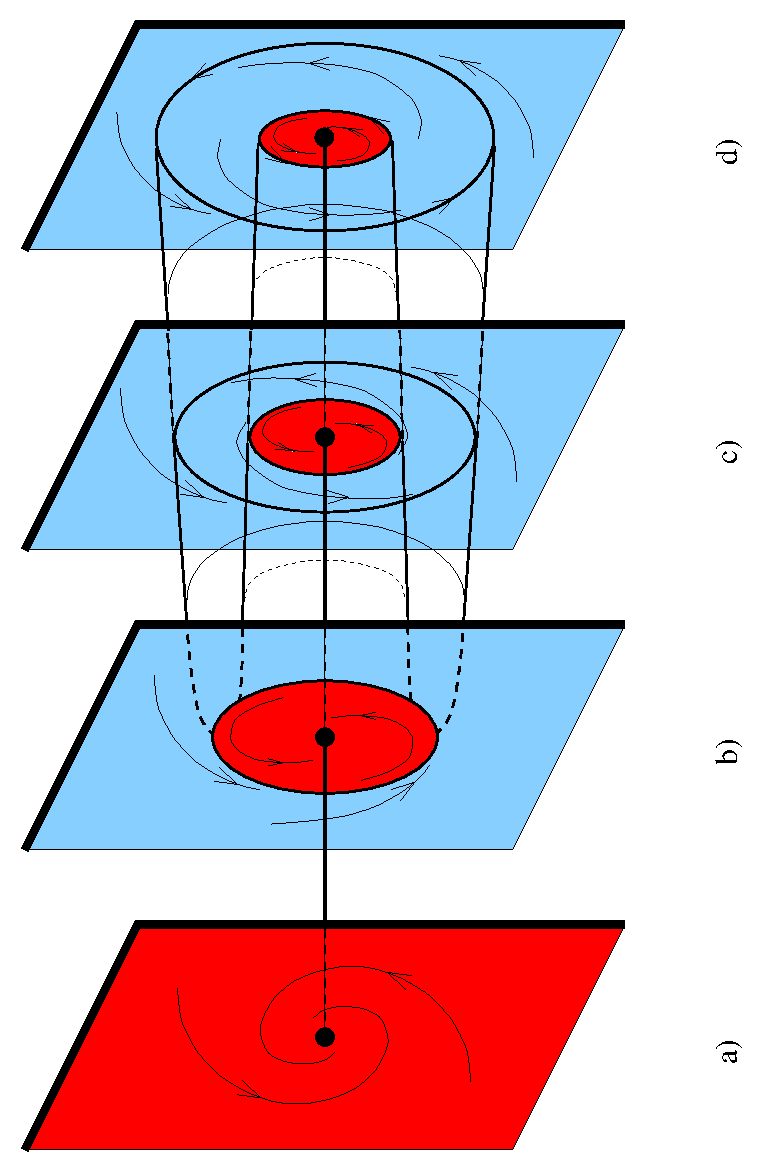
\includegraphics[width=3cm,height=3cm,angle=-90]{figure1}}
\caption{Example of caption of a figure} \label{fig:1}
\end{figure}

\subsection{EQUATIONS}

Equations must be centered and numbered correlatively, leaving
a line between the text and the equation both before and after, or between
two consecutive equations. Reference the equations by their numbering.
\begin{eqnarray}
\mu_A(x) & = & \exp \left( \frac{-(x-\mu_A(x))^2}{2\sigma_A^2} \right)
\end{eqnarray}

\subsection{TABLES}

All tables must be referenced in the text, as
has done in the table~\ref{ttabl}, centered and clear. The number and title
they will always appear at the top of the table, leaving a spacing
of a line between the text of the paragraph and the table. The tables should be
numbered correlatively.

\begin{table}[ht]
\begin{center}
\caption{Example of title of a table.}\label{ttabl}
\begin{tabular}{|c|l|}
   \hline
   {\bf Name} & {\bf Description} \\ \hline $A$ &   Fuzzy subset of $X$\\
   $\mu_{A}$ & Membership function of $A$ \\
   \hline
\end{tabular}
\end{center}
\end{table}

\section*{Acknowledgement}

The word {\bf Acknowledgment} must be aligned to the left,
unnumbered and in bold. All acknowledgments must appear at the end.

\begin{thebibliography}{99}

\bibitem{bibli1} Pedrycz, W., (1993) Fuzzy sets and fuzzy systems,
Research Studies Press, England.

\bibitem{bibli2} Zadeh, L., (1965) ``Fuzzy logic'',
{\em Fuzzy Sets and Systems}, pp 100-106.

\end{thebibliography}

They must be listed in alphabetical order and justified by the corresponding file.

\end{document}
